%  A simple AAU PhD thesis template (collection of papers).
%  2016-08-01 v. 1.3.1
%  Copyright 2012-2016 by Jesper Kjær Nielsen <jkn@es.aau.dk>
%
%  This is free software: you can redistribute it and/or modify
%  it under the terms of the GNU General Public License as published by
%  the Free Software Foundation, either version 3 of the License, or
%  (at your option) any later version.
%
%  This is distributed in the hope that it will be useful,
%  but WITHOUT ANY WARRANTY; without even the implied warranty of
%  MERCHANTABILITY or FITNESS FOR A PARTICULAR PURPOSE.  See the
%  GNU General Public License for more details.
%
%  You can find the GNU General Public License at <http://www.gnu.org/licenses/>.
%
\documentclass[10pt,twoside,openright]{book}
%%%%%%%%%%%%%%%%%%%%%%%%%%%%%%%%%%%%%%%%%%%%%%%%
% Language, Encoding and Fonts
% http://en.wikibooks.org/wiki/LaTeX/Internationalization
%%%%%%%%%%%%%%%%%%%%%%%%%%%%%%%%%%%%%%%%%%%%%%%%
% Select encoding of your inputs. Depends on
% your operating system and its default input
% encoding. Typically, you should use
%   Linux  : utf8 (most modern Linux distributions)
%            latin1 
%   Windows: ansinew
%            latin1 (works in most cases)
%   Mac    : applemac
% Notice that you can manually change the input
% encoding of your files by selecting "save as"
% an select the desired input encoding. 
\usepackage[utf8]{inputenc}
% Make latex understand and use the typographic
% rules of the language used in the document.
\usepackage[danish,english]{babel}
% Use the palatino font
\usepackage{newpxtext}
\linespread{1.05}         % Palatino needs more leading (space between lines)
% Choose the font encoding
% Choose the font encoding
\usepackage[T1]{fontenc}
%%%%%%%%%%%%%%%%%%%%%%%%%%%%%%%%%%%%%%%%%%%%%%%%
% Graphics and Tables
% http://en.wikibooks.org/wiki/LaTeX/Importing_Graphics
% http://en.wikibooks.org/wiki/LaTeX/Tables
% http://en.wikibooks.org/wiki/LaTeX/Colors
%%%%%%%%%%%%%%%%%%%%%%%%%%%%%%%%%%%%%%%%%%%%%%%%
% load a colour package
\usepackage[dvipsnames]{xcolor}
% UniPrint prefers that no colours are used in the template by default.
% However, if you want some colours, then you can easily change the following
\definecolor{aaublue}{RGB}{0,0,0}% black
%\definecolor{aaublue}{RGB}{33,26,82}% dark blue
% The standard graphics inclusion package
\usepackage{graphicx}
% Set up how figure and table captions are displayed
\usepackage{caption}
\captionsetup{%
  font=footnotesize,% set font size to footnotesize
  labelfont=bf % bold label (e.g., Figure 3.2) font
}
% Make the standard latex tables look so much better
\usepackage{array,booktabs}
\usepackage{tabularx}
\usepackage{multirow}
% Enable the use of frames around, e.g., theorems
% The framed package is used in the example environment
\usepackage{framed}
% Create beautiful plots using TikZ and PGFPLOTS
\usepackage{tikz,pgfplots}
%%%%%%%%%%%%%%%%%%%%%%%%%%%%%%%%%%%%%%%%%%%%%%%%
% Mathematics
% http://en.wikibooks.org/wiki/LaTeX/Mathematics
%%%%%%%%%%%%%%%%%%%%%%%%%%%%%%%%%%%%%%%%%%%%%%%%
% Defines new environments such as equation,
% align and split 
\usepackage{amsmath}
% Adds new math symbols
\usepackage{amssymb}
\usepackage{mathtools}

% Use theorems in your document
% The ntheorem package is also used for the example environment
% When using thmmarks, amsmath must be an option as well. Otherwise \eqref doesn't work anymore.
\usepackage[framed,amsmath,amsthm,thmmarks]{ntheorem}

%%%%%%%%%%%%%%%%%%%%%%%%%%%%%%%%%%%%%%%%%%%%%%%%
% Page Layout and appearance
% http://en.wikibooks.org/wiki/LaTeX/Page_Layout
%%%%%%%%%%%%%%%%%%%%%%%%%%%%%%%%%%%%%%%%%%%%%%%%
% Change margins, papersize, etc of the document
\usepackage[
  paperwidth=17cm, % width of a page
  paperheight=24cm, % height of a page
  outer=2.5cm, % right margin on an odd page
  inner=2.5cm, % left margin on an odd page
  top=2.5cm, % top margin
  bottom=2.5cm % bottom margin
  ]{geometry}
% Enable the crop package if you want to print on a4 paer
%\usepackage[a4,cam,center]{crop}
% Modify how \chapter, \section, etc. look
% \renewcommand{\thesection}{\arabic{section}}
% The titlesec package is very configureable
\usepackage{titlesec}
\titleformat*{\section}{\normalfont\Large\bfseries\color{aaublue}}
\titleformat*{\subsection}{\normalfont\large\bfseries\color{aaublue}}
\titleformat*{\subsubsection}{\normalfont\normalsize\bfseries\color{aaublue}}
%\titleformat*{\paragraph}{\normalfont\normalsize\bfseries\color{aaublue}}
%\titleformat*{\subparagraph}{\normalfont\normalsize\bfseries\color{aaublue}}
% Change some default names
\addto\captionsenglish{%this line is required when using the babel package
  % \renewcommand\appendixname{Paper} % change Appendix to Paper
  \renewcommand\bibname{References} % change Bibliography to references
  \renewcommand\figurename{Fig.} % change Figure to Fig.
}

% Change the headers and footers
\usepackage{fancyhdr}
\pagestyle{fancy}
\fancyhf{} %delete everything
\renewcommand{\headrulewidth}{0pt} %remove the horizontal line in the header
\fancyhead[CE]{\color{aaublue}\small\nouppercase\leftmark} %even page - chapter title
\fancyhead[CO]{\color{aaublue}\small\nouppercase\rightmark} %uneven page - section title
\fancyfoot[CE,CO]{\thepage} %page number on all pages
% Do not stretch the content of a page. Instead,
% insert white space at the bottom of the page
\raggedbottom
% Enable arithmetics with length. Useful when
% typesetting the layout.
\usepackage{calc}
% fix the marginpar command so it is always on the correct side
\usepackage{mparhack}
\usepackage{ragged2e}
\usepackage{longtable}
% \usepackage{pbox}

%%%%%%%%%%%%%%%%%%%%%%%%%%%%%%%%%%%%%%%%%%%%%%%%
% Bibliography
% http://en.wikibooks.org/wiki/LaTeX/Bibliography_Management
%%%%%%%%%%%%%%%%%%%%%%%%%%%%%%%%%%%%%%%%%%%%%%%%
% Bibliography for each chapter
% \usepackage[sectionbib]{chapterbib}
% Custom bibliograhy - used in the list of papers
\usepackage[resetlabels]{multibib}
% \usepackage[style=ieee, backend=biber]{biblatex}
% \addbibresource{bib/mybib.bib}

\newcites{main}{References}
\newcites{M}{Main Publications}
\newcites{S}{Publications with a Supervisory Role}
\newcites{O}{Other Publications}
\newcites{A}{References}


\setcounter{tocdepth}{1}
% \renewcommand*{\bibliographyitemlabel}{[\alph{enumiv}]}

% \makeatletter
% \newrobustcmd*{\mknumAlph}[1]{%
%   \begingroup
%   \blx@tempcnta=#1\relax
%   \ifnum\blx@tempcnta>702 %
%   \else
%     \ifnum\blx@tempcnta>26 %
%       \advance\blx@tempcnta\m@ne
%       \divide\blx@tempcnta26\relax
%       \blx@numalph\blx@tempcnta
%       \multiply\blx@tempcnta26\relax
%       \blx@tempcnta=\numexpr#1-\blx@tempcnta\relax
%     \fi
%   \fi
%   \blx@numAlph\blx@tempcnta
%   \endgroup}
% \def\blx@numAlph#1{%
%   \ifcase#1\relax\blx@warning@entry{Value out of range}\number#1\or
%   A\or B\or C\or D\or E\or F\or G\or H\or I\or J\or K\or L\or M\or
%   N\or O\or P\or Q\or R\or S\or T\or U\or V\or W\or X\or Y\or Z\else
%   \blx@warning@entry{Value out of range}\number#1\fi}
% \makeatother

% \DeclareFieldFormat{labelnumber}{\ifkeyword{mine}{\mknumAlph{#1}}{#1}}



% Change [1,2,3,4] into [1-4]
% \usepackage{cite}

%%%%%%%%%%%%%%%%%%%%%%%%%%%%%%%%%%%%%%%%%%%%%%%%
% Misc
%%%%%%%%%%%%%%%%%%%%%%%%%%%%%%%%%%%%%%%%%%%%%%%%
% Add bibliography and index to the table of
% contents
\usepackage{tocbibind}
% Enable subappendices
\usepackage{appendix}
\renewcommand{\setthesection}{\Alph{section}} % remove the chapter numbering
% Add the command \pageref{LastPage} which refers to the
% page number of the last page
\usepackage{lastpage}
% Add notes to in your document
\usepackage[
%  disable, %turn off todonotes
  colorinlistoftodos, %enable a coloured square in the list of todos
  textwidth=2cm, %set the width of the todonotes
  textsize=scriptsize, %size of the text in the todonotes
  ]{todonotes}
\setlength{\marginparwidth}{2cm}

%%%%%%%%%%%%%%%%%%%%%%%%%%%%%%%%%%%%%%%%%%%%%%%%
% Hyperlinks
% http://en.wikibooks.org/wiki/LaTeX/Hyperlinks
%%%%%%%%%%%%%%%%%%%%%%%%%%%%%%%%%%%%%%%%%%%%%%%%
% Enable hyperlinks and insert info into the pdf
% file. Hypperref should be loaded as one of the 
% last packages
\usepackage{hyperref}
\hypersetup{%
	pdfpagelabels=true,%
	plainpages=false,%
	pdfauthor={Author},%
	pdftitle={Title},%
	pdfsubject={Subject},%
	bookmarksnumbered=true,%
	colorlinks=true,%
	citecolor=aaublue,%
	filecolor=aaublue,%
	linkcolor=aaublue,% you should probably change this to black before printing
	urlcolor=aaublue,%
	pdfstartview=FitH%
}

\DeclareMathAlphabet\mathbfcal{OMS}{cmsy}{b}{n} % for paper A

\usepackage{xcolor}
\def\SBcomment[#1]{\textcolor{Red}{#1}}
\def\SWcomment[#1]{\textcolor{Cyan}{#1}}
\def\MDcomment[#1]{\textcolor{Green}{#1}}
\def\SScomment[#1]{\textcolor{Bittersweet}{#1}}

\usepackage{cases}
\usepackage[final]{pdfpages}
\usepackage{textcomp}
\newcommand{\textApprox}{\raisebox{0.5ex}{\texttildelow}}

\usepackage{dirtytalk}
\usepackage{subfig}
\usepackage{algorithm2e, setspace}
\usepackage{tikz}
\tikzset{>=latex}
\tikzstyle{block} = [draw,minimum size=0.5cm]
\usetikzlibrary{math,arrows,positioning,shapes.geometric, decorations.markings}

\usepackage{listings}
\usepackage{courier}
\usepackage{multirow}
\usepackage{xfrac}

\usepackage[most]{tcolorbox}
\usepackage{tabstackengine}
\stackMath
\newenvironment{rightcases}
  {\left.\begin{alignedat}{2}}
  {\end{alignedat}\right\rbrace}

  \newcommand\norm[1]{\left\lVert#1\right\rVert}

\def\eqrefMatlab[#1]{%
    \hypersetup{linkcolor=[HTML]008400}%
    \color[HTML]{008400}{\texttt{(\ref{#1}})}
}
\def\refMatlab[#1]{%
    \hypersetup{linkcolor=[HTML]008400}%
    \color[HTML]{008400}{\texttt{\ref{#1}}}}


\renewcommand{\lstlistingname}{Algorithm}% 
\def\setlstCpp
{
  \lstset{ %
  backgroundcolor=\color{black!0},   % choose the background color; you must add \usepackage{color} or \usepackage{xcolor}
  basicstyle=\footnotesize\ttfamily,        % the size of the fonts that are used for the code
  breakatwhitespace=true,         % sets if automatic breaks should only happen at whitespace
  breaklines=true,                 % sets automatic line breaking
  captionpos=b,                    % sets the caption-position to bottom
  commentstyle=\color[HTML]{008400},    % comment style
  % escapeinside={\%*}{*)},          % if you want to add LaTeX within your code
  extendedchars=true,              % lets you use non-ASCII characters; for 8-bits encodings only, does not work with UTF-8
  frame=tb,	                   	   % adds a frame around the code
  keepspaces=true,                 % keeps spaces in text, useful for keeping indentation of code (possibly needs columns=flexible)
  keywordstyle=\color[HTML]{B82BA1},       % keyword style
  language=C++,                 % the language of the code (can be overrided per snippet)
  % otherkeywords={*,...},           % if you want to add more keywords to the set
  numbers=none,                    % where to put the line-numbers; possible values are (none, left, right)
  numbersep=5pt,                   % how far the line-numbers are from the code
  numberstyle=\tiny\color{black},%\noncopynumber, % the style that is used for the line-numbers
  rulecolor=\color{black},         % if not set, the frame-color may be changed on line-breaks within not-black text (e.g. comments (green here))
  showspaces=false,                % show spaces everywhere adding particular underscores; it overrides 'showstringspaces'
  showstringspaces=false,          % underline spaces within strings only
  showtabs=false,                  % show tabs within strings adding particular underscores
  stepnumber=1,                    % the step between two line-numbers. If it's 1, each line will be numbered
  stringstyle=\color[HTML]{D12F1B}, % string literal style
  tabsize=2,	                   % sets default tabsize to 2 spaces
  title=\lstname,                  % show the filename of files included with \lstinputlisting; also try caption instead of title
  columns=fixed,                    % Using fixed column width (for e.g. nice alignment),
  deletekeywords={*, float},            % if you want to delete keywords from the given language
  }
}

\def\setlstMAT
{
  \lstset{ %
    backgroundcolor=\color[HTML]{FCFDDB},   % choose the background color; you must add \usepackage{color} or \usepackage{xcolor}
    basicstyle=\footnotesize\ttfamily,        % the size of the fonts that are used for the code
    breakatwhitespace=false,         % sets if automatic breaks should only happen at whitespace
    breaklines=true,                 % sets automatic line breaking
    captionpos=b,                    % sets the caption-position to bottom
    commentstyle=\color[HTML]{008400},    % comment style
    escapeinside={\%*}{*)},          % if you want to add LaTeX within your code
    extendedchars=true,              % lets you use non-ASCII characters; for 8-bits encodings only, does not work with UTF-8
    frame=tb,	                   	   % adds a frame around the code
    keepspaces=true,                 % keeps spaces in text, useful for keeping indentation of code (possibly needs columns=flexible)
    keywordstyle=\color[HTML]{0000FF},       % keyword style
    language=MATLAB,                 % the language of the code (can be overrided per snippet)
    otherkeywords={...},           % if you want to add more keywords to the set
    numbers=left,                    % where to put the line-numbers; possible values are (none, left, right)
    numbersep=5pt,                   % how far the line-numbers are from the code
    numberstyle=\tiny\color{black},%\noncopynumber, % the style that is used for the line-numbers
    rulecolor=\color{black},         % if not set, the frame-color may be changed on line-breaks within not-black text (e.g. comments (green here))
    showspaces=false,                % show spaces everywhere adding particular underscores; it overrides 'showstringspaces'
    showstringspaces=false,          % underline spaces within strings only
    showtabs=false,                  % show tabs within strings adding particular underscores
    stepnumber=1,                    % the step between two line-numbers. If it's 1, each line will be numbered
    stringstyle=\color[HTML]{A100F4}, % string literal style
    tabsize=2,	                   % sets default tabsize to 2 spaces
    title=\lstname,                  % show the filename of files included with \lstinputlisting; also try caption instead of title
    columns=fixed,                   % Using fixed column width (for e.g. nice alignment)
    deletekeywords={pi, zeros, plot, round, ceil, floor, cos, sin, sum, abs, eps, exp, toeplitz, eye, min, max, reshape, kron, speye, sqrt, sparse, ls, amp},            % if you want to delete keywords from the given language
    morestring=[b]"
  }
}% package inclusion and set up of the document
% see, e.g., http://en.wikibooks.org/wiki/LaTeX/Formatting#Hyphenation
% for more information on word hyphenation
\hyphenation{ex-am-ple hy-phen-a-tion short}
\hyphenation{long la-tex}
% 
% see, e.g., http://en.wikibooks.org/wiki/LaTeX/Customizing_LaTeX#New_commands
% for more information on how to create macros

%%%%%%%%%%%%%%%%%%%%%%%%%%%%%%%%%%%%%%%%%%%%%%%%
% Macros for the titlepage
%%%%%%%%%%%%%%%%%%%%%%%%%%%%%%%%%%%%%%%%%%%%%%%%
%Creates the aau titlepage
\newcommand{\aautitlepage}[3]{%
  {
    %set up various length
    \ifx\titlepageleftcolumnwidth\undefined
      \newlength{\titlepageleftcolumnwidth}
      \newlength{\titlepagerightcolumnwidth}
    \fi
    \setlength{\titlepageleftcolumnwidth}{0.5\textwidth-\tabcolsep}
    \setlength{\titlepagerightcolumnwidth}{\textwidth-2\tabcolsep-\titlepageleftcolumnwidth}
    %create title page
    \thispagestyle{empty}
    \noindent%
    \begin{tabular}{@{}ll@{}}
      \parbox{\titlepageleftcolumnwidth}{
        \iflanguage{danish}{%
          
\includegraphics[width=\titlepageleftcolumnwidth]{AAUgraphics/aau_logo_da}
        }{%
          
\includegraphics[width=\titlepageleftcolumnwidth]{AAUgraphics/aau_logo_en}
        }
      } &
      \parbox{\titlepagerightcolumnwidth}{\raggedleft\sf\small
        #2
      }\bigskip\\
       #1 &
      \parbox[t]{\titlepagerightcolumnwidth}{%
      \textbf{Abstract:}\bigskip\par
        \fbox{\parbox{\titlepagerightcolumnwidth-2\fboxsep-2\fboxrule}{%
          #3
        }}
      }\\
    \end{tabular}
    \vfill
    \iflanguage{danish}{%
      \noindent{\footnotesize\emph{Rapportens indhold er frit tilgængeligt, men offentliggørelse (med kildeangivelse) må kun ske efter aftale med forfatterne.}}
    }{%
      \noindent{\footnotesize\emph{The content of this report is freely available, but publication (with reference) may only be pursued due to agreement with the author.}}
    }
    \clearpage
  }
}

%Create english project info
\newcommand{\englishprojectinfo}[8]{%
  \parbox[t]{\titlepageleftcolumnwidth}{
    \textbf{Title:}\\ #1\bigskip\par
    \textbf{Theme:}\\ #2\bigskip\par
    \textbf{Project Period:}\\ #3\bigskip\par
    \textbf{Project Group:}\\ #4\bigskip\par
    \textbf{Participant(s):}\\ #5\bigskip\par
    \textbf{Supervisor(s):}\\ #6\bigskip\par
    \textbf{Copies:} #7\bigskip\par
    \textbf{Page Numbers:} \pageref{LastPage}\bigskip\par
    \textbf{Date of Completion:}\\ #8
  }
}

%Create danish project info
\newcommand{\danishprojectinfo}[8]{%
  \parbox[t]{\titlepageleftcolumnwidth}{
    \textbf{Titel:}\\ #1\bigskip\par
    \textbf{Tema:}\\ #2\bigskip\par
    \textbf{Projektperiode:}\\ #3\bigskip\par
    \textbf{Projektgruppe:}\\ #4\bigskip\par
    \textbf{Deltager(e):}\\ #5\bigskip\par
    \textbf{Vejleder(e):}\\ #6\bigskip\par
    \textbf{Oplagstal:} #7\bigskip\par
    \textbf{Sidetal:} \pageref{LastPage}\bigskip\par
    \textbf{Afleveringsdato:}\\ #8
  }
}

%%%%%%%%%%%%%%%%%%%%%%%%%%%%%%%%%%%%%%%%%%%%%%%%
% An example environment
%%%%%%%%%%%%%%%%%%%%%%%%%%%%%%%%%%%%%%%%%%%%%%%%
\theoremheaderfont{\normalfont\bfseries}
\theorembodyfont{\normalfont}
\theoremstyle{break}
\def\theoremframecommand{{\color{gray!50}\vrule width 5pt \hspace{5pt}}}
\newshadedtheorem{exa}{Example}[chapter]
\newenvironment{example}[1]{%
		\begin{exa}[#1]
}{%
		\end{exa}
}
% my new macros

\begin{document}
%frontmatter
\frontmatter
\pagestyle{empty} %disable headers and footers
\pagenumbering{roman} %use roman page numbering in the frontmatter
\pdfbookmark[0]{Front page}{label:frontpage}%
\begin{titlepage}
  \addtolength{\hoffset}{0.5\evensidemargin-0.5\oddsidemargin} %set equal margins on the frontpage - remove this line if you want default margins
  \noindent%
  \begin{tabular}{@{}p{\textwidth}@{}}
    \toprule[2pt]
    \midrule
    \vspace{0.2cm}
    \begin{center}
      {\fontsize{23pt}{24pt}\selectfont\textbf{
      The Emulated Ensemble}}\\
      \vspace{0.5cm}\Large{Real-Time Simulation of Musical Instruments using Finite-Difference Time-Domain Methods}
    \end{center}
    \vspace{0.2cm}\\
    \midrule
    \toprule[2pt]
  \end{tabular}
  \vspace{4 cm}
  \begin{center}
    {\large
      Ph.D. Dissertation%Insert document type (e.g., Project Report)
    }\\
    \vspace{0.2cm}
    {\Large
      Silvin Willemsen%Insert your group name or real names here
    }
  \end{center}
  \vfill
  \begin{center}
  Dissertation submitted \today
  \end{center}
\end{titlepage}
\clearpage

\thispagestyle{empty}
\noindent
% \fontsize{9.5}{12}\selectfont % so that the department fits on the line
\begin{tabularx}{\textwidth}{@{}lX}
    Thesis submitted: & \today\\
    \\
    PhD Supervisor: & Prof.\ Stefania Serafin\\
                    & Aalborg University\\
                    \\
    Co-Supervisor (external): & Prof.\ Stefan Bilbao\\
                    & University of Edinburgh\\
                    \\
    PhD Committee:  & Assoc. Prof. Olga Timcenko\\
                    & Aalborg University\\
                    \\
                    & Prof. Julius O. Smith III \\
                    & Stanford University\\
                    \\
                    & Prof. Augusto Sarti\\
                    & Politecnico di Milano\\
                   \\
    PhD Series:    & Technical Faculty of IT and Design, Aalborg University\\
    \\
    Department: & Department of Architecture, Design and Media Technology
\end{tabularx}
% \normalsize
\strut\vfill
\noindent
\begin{tabularx}{\textwidth}{@{}lX}
    ISSN: & xxxx-xxxx\\
    ISBN: & xxx-xx-xxxx-xxx-x\\
\end{tabularx}
\strut\vfill
\noindent Published by:\newline
Aalborg University Press\newline
Skjernvej 4A, 2nd floor\newline
DK – 9220 Aalborg Ø\newline
Phone: +45 99407140\newline
aauf@forlag.aau.dk\newline
forlag.aau.dk
\strut\vfill
\noindent \copyright{} Copyright: Silvin Willemsen\newline
\strut\vfill
\noindent Printed in Denmark by Rosendahls, 2021
\clearpage


% mainfile: ../master.tex
\chapter*{Author CV\markboth{Author CV}{Author CV}}\label{ch:cv}
\pagestyle{fancy}
% \addcontentsline{toc}{chapter}{Curriculum Vitae}
% \begin{tabularx}{\textwidth}{@{}Xr}
%     \Large Silvin Willemsen & \raisebox{-\totalheight/2}{
\includegraphics[width=2cm]{frontmatter/cvPicture.png}}\\
% \end{tabularx}\par
% \vspace{0.5cm}\noindent
Silvin Willemsen received his BSc. in Industrial Design from Eindhoven  University of Technology in 2015 and his MSc. in Sound and Music Computing from Aalborg University in 2017. In 2018, he was appointed as a PhD Stipend at the Department of Architecture, Design and Media Technology at Aalborg University Copenhagen and was affiliated with the Multisensory Experience Lab. During the PhD project he supervised students following the Sound and Music Computing master's programme, and was involved with teaching the courses \textit{Physical Modelling for Sound Synthesis} and \textit{Sound Processing}.
% mainfile: ../master.tex
\chapter*{Abstract\markboth{Abstract}{Abstract}}\label{ch:Abstract}
\addcontentsline{toc}{chapter}{Abstract}
Over the past few decades, numerous strategies to virtualise traditional instruments have been developed. Although one could create digital musical instruments using pre-recorded samples of their real-life counterparts, the playability will not be captured. Instead, a simulation of the underlying physics of the instrument could be created, and is much more flexible to player interaction. This \textit{physical model} will allow a musician to be much more expressive when playing the digital instrument than if static samples were to be used. Using ad hoc hardware to control the simulation could potentially make the simulated instrument feel identical to the original.

% Physical models can be used to simulate traditional musical instruments that are too rare or valuable to be played. These cases 

% Furthermore, 
Applications of physical modelling for musical instruments include simulating instruments that are unplayable as they are too rare or vulnerable. A model of the underlying physics of the instrument could potentially resurrect the instrument making it available to the public again. 
Furthermore, as a simulation is not restricted by the laws of physics, one could extend the possibilities of the original instrument. Properties such as the material or geometry of an instrument could be dynamically changed which broadens the range of expression of the musician. One could even imagine physically impossible musical instruments which still exhibit a natural sound due to the underlying models.

In this project, finite-difference time-domain (FDTD) methods have been chosen, as they have an advantage in terms of generality and flexibility regarding the systems they can model. A drawback of these methods is that they are quite computationally expensive, and although many highly accurate models based on these methods have existed for years, the computing power to run them in real time has only recently become available. The main challenge %introduced by these methods 
% and physical modelling in general are: 
% \begin{enumerate}
%     \item the underlying physical model needs to be formulated, which gets increasingly complex for higher accuracy, and
%     \item  
is thus to run the simulations in real time to allow for proper player interaction.

This thesis presents the development and real-time implementation of various physical models of traditional musical instruments based on FDTD methods. These instruments include the trombone and more obscure instruments such as the hurdy gurdy and the tromba marina. Furthermore, a novel method is presented that paves the way for dynamic FDTD-based musical instrument simulations allowing for physically impossible instrument manipulations. Finally, this work doubles as an aid for beginners in the field of musical instrument simulations based on FDTD methods, and aims to provide a low-entry-level explanation of the literature and theory that the physical models are based on. 

\chapter*{Resum{\'e}\markboth{Resum{\'e}}{Resum{\'e}}}\label{ch:Resume}
\addcontentsline{toc}{chapter}{Resum{\'e}}
I l{\o}bet af de sidste {\aa}rtier, er der blevet udviklet adskillige strategier til at lave virtuelle udgaver af traditionelle musikinstrumenter. Selvom digitale musikinstrumenter baseret p{\aa} traditionelle musikinstrumenter, kan skabes ved hj{\ae}lp af lydoptagelser af deres virkelige modstykke, er det ofte p{\aa} bekostning instrumenternes spilbarhed.
En anden strategi ville v{\ae}re at implementere en digital simulering af instrumentets underliggende fysik, hvilket ville give en mere fleksibel og naturlig interaktion. Denne digitale simulering, en fysisk model af instrumentet, ville g{\o}re det muligt for en musiker at v{\ae}re mere udtryksfuld n{\aa}r han eller hun spiller p{\aa} det digitale musikinstrument end med statiske lydoptagelser. Derudover, ved at bruge ad hoc hardware til at styre simuleringen, kunne man potentielt f{\aa} det digitale musikinstrument til at f{\o}les identisk med originalen. 

Fysisk modellering af musikinstrumenter kan ogs{\aa} anvendes til at simulere musikinstrumenter, der er sj{\ae}ldne eller for s{\aa}rbare til at m{\aa} spilles p{\aa}. Her ville en model af instrumentets underliggende fysik potentielt kunne genoplive instrumentet ved g{\o}re det tilg{\ae}ngeligt og spilbart igen. Ydermere, kunne man forbedre det originale instrument, eftersom en digital simulering ikke er begr{\ae}nset af fysikkens love. Egenskaber som instruments materiale eller geometri kunne dynamisk {\ae}ndres og udvide musikerens udtryksmuligheder. Man kunne endda forestille sig fysisk umulige musikinstrumenter, der stadig har en naturlig klang p{\aa} grund af de underliggende modelleringsprincipper. 

Til dette projekt er finite-difference time-domain (FDTD) metoderne blevet valgt som modelleringsteknik, siden disse metoder er generelle og fleksible og derfor har en fordel i forhold til de forskellige typer af systemer som de kan modellere.  En ulempe ved FDTD metoderne er at de er beregningstunge, og selvom der har eksisteret n{\o}jagtige modeller baseret p{\aa} disse metoder i {\aa}revis, er computer regnekraften til at k{\o}re dem i realtid f{\o}rst blevet tilg{\ae}ngelig for nyligt. Den st{\o}rste udfordring er derfor at k{\o}re simuleringerne i realtid og at opn{\aa} naturlig interaktion imellem ud{\o}veren og simuleringen. 

Denne afhandling beskriver udviklingen og implementeringen af forskellige fysiske modeller af traditionelle musikinstrumenter baseret p{\aa} FDTD metoder i realtid. Disse instrumenter inkluderer trombone og mindre kendte instrumenter som drejelire og tromba marina. Desuden pr{\ae}senteres en ny metode, der muligg{\o}r dynamiske parametre i FDTD-baserede musikinstrumentsimuleringer og tillader instrumentmanipulationer som er umulige i den virkelige verden. 
Derudover, kan denne afhandling bruges som et hj{\ae}lpemiddel til begyndere inden for simuleringer af musikinstrumenter, og sigter mod at give en begyndervenlig forklaring af den litteratur og teori, som de fysiske modeller er baseret p{\aa}. 

\cleardoublepage
\pdfbookmark[0]{Contents}{label:contents}
\pagestyle{fancy} %enable headers and footers again
\tableofcontents
\listoftodos
% mainfile: ../master.tex
\chapter*{Preface\markboth{Preface}{Preface}}\label{ch:preface}
\pagestyle{fancy}
\addcontentsline{toc}{chapter}{Preface}

Starting this PhD project, I did not have a background in mathematics, physics or computer science, which were three equally crucial components in creating the result of this project. After the initial steep learning curve of notation and terminology, I was surprised to find that the methods used for physical modelling are actually quite straightforward! 

Of course it should take a bit of time to learn these things, but 



Many concepts that seemed impossible at the beginning 

I feel that the literature lacks a lot of the intuition needed for readers without a background in any of these topics. Rather, much of the literature I came across assumes that the reader has a degree in at least one of the aforementioned topics. Stefan Bilbao's seminal work \textit{Numerical Sound Synthesis}, which is the most complete work to date describing how to physically model musical instruments using finite-difference time-domain methods says that "A strong background in digital signal processing, physics, and computer programming is essential."
Even though some basic calculus knowledge is assumed to understand the concepts used in this work, a degree in any of the aforementioned topics is (hopefully) unnecessary. \SWcomment[Furthermore, some experience with MATLAB and C++ is assumed for the code examples]

Some working titles: \textit{Physical Modelling for Dummies} \textit{Physical Modelling for the faint-hearted}

Also, I came across a lot of ``it can be shown that's without derivations. This is why I decided to write this work a bit more pedagogical, and perhaps more elaborate than what could be expected. 

I believe that anyone with some basic skills in mathematics and programming is able to create a simulation based on physics within a short amount of time, given the right tools, which I hope that this dissertation could be.  

The knowledge dissemination of this dissertation is thus not only limited to the research done and publications made over the course of the project, but also its pedagogical nature hopefully allowing future (or past) students to benefit from.

As with a musical instrument itself, a low entry level, a gentle learning curve along with a high virtuosity level is desired. Take a piano, for instance. Most will be able to learn a simple melody — such as “Fr\`ere Jacques” — in minutes, but to become virtuous requires years of practice.

This is the way I wanted to write this dissertation: easy to understand the basic concepts, but many different aspects touched upon to allow for virtuosity. Hopefully by the end, the reader will at least grasp some highly complex concepts in the fields of mathematics, physics and computer science (which will hopefully take less time than it takes to become virtuous at playing the piano). 

As Smith states in his work \textit{Physical Audio Signal Processing} \cite{Smith2010b} ``All we need is Newton'', and indeed, all Newton's laws of motion will make their appearance in this document.


I wanted to show my learning process and (hopefully) explain topics such as \textit{Energy Analysis}, \textit{Stability Analysis}, etc. in a way that others lacking the same knowledge %(/ with the same background) 
will be able to understand.

Make physical modelling more accessible to the non-physicist. Also supports reproducibility of science and lowers the entry level   


\textit{Interested in physically impossible manipulations of now-virtual instruments.}


\SWcomment[Could be fun to include this :) :] ``I'm a musician. Will I be out of a job if you keep making physical models?'' Physical modelling is not here to replace the original instruments and the musicians playing them. Instead, it can be used as a tool to understand the physics of existing instruments and possibly go beyond. Simulated instruments are not restricted by physics anymore and could provide new ways of expression for the musician.

\subsubsection{Acknowledgements}

I would like to thank my mom..

First and foremost, I want to wholeheartedly like to thank my supervisor and friend Stefania Serafin, without whom none of this would have been possible. After she approached me 

I quickly found out that this project was a ``golden ticket'' to go in whichever direction I wanted to as long as it is publishable. She provided this opportunity and let me be free in my decisions throughout my project and I am extremely grateful for that.

Next, I would like to thank Stefan Bilbao for his invaluable help throughout this PhD project. He has been an incredible mentor and the results of this project would not have been possible without him.  been an incredible help


and his seminal work \textit{Numerical Sound Systhesis} have been invaluable to the result of this project...
Michele Ducceschi

% Other guys at Edinburgh: Brian, Charlotte, Craig

I would like to thank Madeleine Koudstaal, Marius Onofrei, Razvan Paisa, Nikolaj Andersson, Pelle Juul Christensen

Colleagues and friends from the Multisensory Experience Lab
, Pelle Juul Christensen, Nikolaj Andersson, Razvan Paisa, Ali Adjorlu, Lars Andersen, Nicklas Andersen, Karolina Prawda, Nathalie, Anca-Simona Horvath, Mauro Nascimben, Rares Stefan Alecu, Titas Lasickas, Vesa V{\"a}lim{\"a}ki

% James, Jerome, Federico Fontana, Romain, 

Finally, I would like to thank my family for having always supported the decisions I made and providing the freedom I needed to pursue my dreams. Specifically, I would like to thank Anna

% Anna, who has always been willing to sit through my try-out lectures and conference presentations and  headaches from unfinished (and finished) implementations. 

\vfill
\hfill Silvin Willemsen

\hfill Copenhagen, \today

\cleardoublepage

%mainmatter
\mainmatter
\custPart{Introduction}\label{part:introduction}
\chapter*{Resonators}
<<<<<<< HEAD
Though the physical models described in the previous part are also considered resonators, they are \textit{ideal} cases. In other words, you would not be able to find these ``in the wild'' as they do not includes effects such as losses or frequency dispersion. 

This part presents the different resonators used over the course of the project and is structured as follows: Chapter \ref{ch:stiffString} introduces the stiff string, a model which has been used a lot over the course of this project, Chapter \ref{ch:brass} talks about brass instruments, or more generally, 1D systems of varying geometry along their spatial dimension. Finally, Chapter \ref{ch:2Dsyst} will introduces 2D systems which, in this project, have been used to simulate (simplified) instrument bodies.
=======
Although the physical models described in the previous part -- the simple mass-spring system and the 1D wave equation -- are also considered resonators, they are \textit{ideal} cases. In other words, these can not be found in the real world as effects such as losses or frequency dispersion are not included. 

This part presents the different resonators used over the course of the project that better include these non-ideal physical processes and is structured as follows: Chapter \ref{ch:stiffString} introduces the stiff string, an extension of the 1D wave equation, % and is the single most-used model in this project. 
Chapter \ref{ch:brass} introduces acoustic tubes, used to model brass instruments, and finally, Chapter \ref{ch:2Dsyst} introduces 2D systems which, in this project, have been used to simulate (simplified) instrument bodies. The analysis techniques introduced in the previous part will be applied to all models and described in detail. 
>>>>>>> master


\custPart{Models}
\newcommand{\modelstitle}{Models}
\chapter*{\modelstitle}\label{sec:models}
\addcontentsline{toc}{chapter}{\modelstitle}

\chapter*{Resonators}
<<<<<<< HEAD
Though the physical models described in the previous part are also considered resonators, they are \textit{ideal} cases. In other words, you would not be able to find these ``in the wild'' as they do not includes effects such as losses or frequency dispersion. 

This part presents the different resonators used over the course of the project and is structured as follows: Chapter \ref{ch:stiffString} introduces the stiff string, a model which has been used a lot over the course of this project, Chapter \ref{ch:brass} talks about brass instruments, or more generally, 1D systems of varying geometry along their spatial dimension. Finally, Chapter \ref{ch:2Dsyst} will introduces 2D systems which, in this project, have been used to simulate (simplified) instrument bodies.
=======
Although the physical models described in the previous part -- the simple mass-spring system and the 1D wave equation -- are also considered resonators, they are \textit{ideal} cases. In other words, these can not be found in the real world as effects such as losses or frequency dispersion are not included. 

This part presents the different resonators used over the course of the project that better include these non-ideal physical processes and is structured as follows: Chapter \ref{ch:stiffString} introduces the stiff string, an extension of the 1D wave equation, % and is the single most-used model in this project. 
Chapter \ref{ch:brass} introduces acoustic tubes, used to model brass instruments, and finally, Chapter \ref{ch:2Dsyst} introduces 2D systems which, in this project, have been used to simulate (simplified) instrument bodies. The analysis techniques introduced in the previous part will be applied to all models and described in detail. 
>>>>>>> master

\section{To do thingies}\label{sec:ch2label}
\begin{itemize}
  \item Think about how to define real-time.
  \item Create an intuition for different parts of the equation
  \item Talk about input and output locations and how that affects frequency content (modes).
\end{itemize}

\subsection{Intuition for the frequency dependent damping term}
Take the frequency independent damping term $-2\sigma_0\partial_tu$. The more positive the velocity $\partial_tu$ is, i.e., the string is moving upwards the more this term applies a negative, or downwards force (/effect) on the string. Vice versa, a more negative velocity will make this term apply a more positive force on the string. As for the frequency dependent damping term, apart from the obvious $\sigma_1$, the effect of the term increases with an increase of $\partial_t\partial_x^2u$ which describes the rate of change of the curvature of the string.

Let's first talk about positive and negative curvature, i.e., when $\partial_x^2u > 0$ or $\partial_x^2u < 0$. Counterintuitively, in the positive case, the curve points downwards. Think about the function $f(x) = x^2$. It has a positive curvature (at any point), but has a minimum. We can prove this by taking $x=0$ and setting grid spacing $h=1$.
\begin{equation}
  \begin{aligned}
  \delta_{xx}f(x) &= \frac{1}{h^2} \left(f(-1)-2f(0)+f(1)\right), \\
  &= \frac{1}{1^2} \left((-1)^2-2\cdot0^2+1^2\right),\\
  &= \left(1-0+1\right) = 2.
  \end{aligned}
\end{equation}
In other words, the second derivative of the function $f(x)=x^2$ around $x=0$ is positive.

As our term does not only include a second-order spatial derivative but also a first-order time derivative, we are now talking about a positive or negative \textit{rate of change} of the curvature, i.e., when $\partial_t\partial_x^2u>0$ or $\partial_t\partial_x^2u<0$. A positive rate of change of curvature means that the string either has a positive curvature and is getting more positive, i.e., the string gets more curved over time, or that the string has a negative curvature and is getting less negative, i.e., the string gets less curved or 'loosens up' over time.  In the same way, a negative rate of change of curvature means that the string either has a negative curvature and is getting more negative, or that the string has a positive curvature and is getting less positive. 

Let's see some examples. Take the same function described before, but now $f$ changes over time, fx. $f(x, t)=tx^2$. When $t$ increases over time, the curvature gets bigger. Repeating what we did above with $x=0$ and grid spacing $h = 1$, but now with $t=2$ and step size $k=1$, but now with a backwards time derivative we get:
  \begin{alignat*}{3}
    \delta_{t-}\delta_{xx}f(x,t) &= \frac{1}{kh^2}\bigg(&&f(-1, 2) - 2f(0, 2) + f(1, 2) \\
    & &&- \Big(f(-1, 1) - 2f(0, 1) + f(1, 1)\Big)\bigg),\\
    & = \frac{1}{1\cdot 1^2}\bigg(&&2\cdot(-1)^2-2\cdot2\cdot(0)^2+2\cdot1^2\\
    & &&-\Big(1\cdot(-1)^2-2\cdot1\cdot(0)+1\cdot(1^2)\Big)\Bigg),\\
    &=2+2-&&(1+1)=2.
  \end{alignat*}
So the rate of change of the curvature is positive, i.e., the already positively curved function $x^2$ gets more curved over time.

If the curvature around a point along a string gets more positive (or less negative) over time, the force applied to that point will be positive. Vice versa, if the curvature around a point along a string gets more negative (or less positive) over time, the force applied will be negative.
 
The fact the frequency dependent term to be added rather than subtracted to the FDS, is caused by the fact that a positive curvature implies a negative position in the string (think of the function $x^2$ which has a positive curvature, but the function `points' downwards). This translated to the force/effect this term has on the scheme means...

\section{Discussion and Conclusion}\label{sec:conclusion}


% {\small\bibliographystyle{IEEEtranS}\bibliography{bib/mybib}}


\custPart{Dynamic Grids}
\chapter{Dynamic Grid}\label{ch:dynamicGrid}

\textit{Often in math, you should view the definition not as a starting point, but as a target. Contrary to the structure of textbooks, mathematicians do not start by making definitions and then listing a lot of theorems, and proving them, and showing some examples. The process of discovering math typically goes the other way around. They start by chewing on specific problems, and then generalising those problems, then coming up with constructs that might be helpful in those general cases,and only then you write down a new definition (or extend an old one). - Grant Sanderson (AKA 3Blue1Brown) https://youtu.be/O85OWBJ2ayo?t=359}

This chapter provides an extended summary to the paper ``Dynamic grids for Finite-Difference Schemes in Musical Instrument Simulations'' \citeP[G]. The paper presents a novel method to smoothly add and remove grid points from a FD scheme which allows for dynamic parameter variations without compromising stability or quality of the simulation (see Section \ref{sec:quality1DWave}). 

After a brief introduction  and summary of the method, the chapter will extend on paper \citeP[G] by providing some design considerations as a result of iterations done as well as providing details on the implementation of the displacement correction and the modal analysis shown in the paper. 

\section{Background and motivation}
Simulating musical instruments using physical modelling -- as mentioned in Chapter \ref{ch:physMod} -- allows for manipulations of the instrument that are impossible in the physical world. Examples of this are changes in material density or stiffness, cross-sectional area (1D), thickness (2D) and size of the system in general. 



\subsection{Examples}
Apart from being potentially sonically interesting, there are examples in the physical world where certain aspects of the instrument are manipulated in real-time.

Tension in a string is changed when tuning it

Some artists even use this in their performances \cite{Gomm2011, Mayer2008}
Or gr4yhound: https://www.youtube.com/watch?v=fSQ9Dg65EFo

The hammered dulcimer is another example where the strings are tensioned over a bridge where one can play the string at one side of the bridge, while pushing down on the same string on the other side \cite{Glenn2014}.

\noindent 1D:
\begin{itemize}
    \item Trombone
    \item Slide whistle
    \item Guitar strings
    \begin{itemize}
        \item Fretting finger pitch bend
        \item Above the nut \cite{Mayer2008}
        \item Tuning pegs directly \cite{Gomm2011}
    \end{itemize}
    \item Hammered dulcimer \cite{Glenn2014}
    \item Erhu? 
\end{itemize}
%
2D: 
\begin{itemize}
    \item Timpani
    \item Bodhr\'an: https://youtu.be/b9HyB5yNS1A?t=146
    \item Talking drum (hourglass drum): https://youtu.be/B4oQJZ2TEVI?t=9
    \item Flex-a-tone (could also be 1D tbh..): https://www.youtube.com/watch?v=HEW1aG8XJQk.
\end{itemize}

A more relevant example is that of the trombone, where the size of the instrument is changed in order to play different pitches. Modelling this using FDTD methods would require

% \section{Issues with FDTD methods}


In his thesis, Harrison points out that in order to model the trombone, grid points need to be introduced 


Something about time-dependent variable coefficient Stokes flow:
https://arxiv.org/abs/1010.2832

Time-varying propagation speed in waveguides: https://quod.lib.umich.edu/cgi/p/pod/dod-idx/fractional-delay-application-time-varying-propagation-speed.pdf?c=icmc;idno=bbp2372.1997.069;format=pdf

Special boundary conditions (look at!):
Modeling of Complex Geometries and Boundary Conditions in Finite Difference/Finite Volume Time Domain Room Acoustics Simulation (\url{https://www.researchgate.net/publication/260701231_Modeling_of_Complex_Geometries_and_Boundary_Conditions_in_Finite_DifferenceFinite_Volume_Time_Domain_Room_Acoustics_Simulation})



\section{Summary}
The variations are assumed to be at sub-audio rate (i.e., human gestural control) so that analysis techniques are still valid to some degree.


Consider the 1D wave equation  as presented in Section \ref{sec:1DWave}, describing the motion of a system of length $L$, its state described by $q = q(x,t)$ defined for $t\geq 0$ and $x\in\D$ with domain $\D = [0, L]$. This state variable can be discretised to a grid function $\qln$ with $n\in \mathbb{N}^0$ and $l \in \{0, \hdots, N\}$ with $N$ being tthe number of intervals between the grid points. The PDE in \eqref{eq:1DwavePDE} can then be discretised to the following FD scheme
\begin{equation}
    \dtt \qln = c^2\dxx \qln.
\end{equation}

Rather than working with this scheme directly, paper \citeP[G] proposes to split it into two to get the following system 
\begin{subequations}
    \begin{equation}
        \dtt \ulun = c^2\dxx \ulun,
        \dtt \wlwn = c^2\dxx \wlwn.
    \end{equation}
\end{subequations}

\section{Iterations}
Iterations have been:
\begin{itemize}
    \item Interpolated boundary conditions
    \item Linear interpolation
\end{itemize}

\todo{These sections are taken from the JASA appendix} In this appendix, some iterations done over the course of this project will be shown in more detail. In the following, the 1D wave equation with a wave speed of $c = 1470$ m/s, a length of $L = 1$ m, Dirichlet boundary conditions and a sample rate of $f_\text{s} = 44100$ Hz is considered, and -- through Eq. \eqref{eq:compactLambda} -- satisfies the CFL condition with equality. These values result in $N = 30$, or a grid of 31 points including the boundaries. Then, the wave speed is decreased to $c \approx 1422.6$ m/s, i.e., the wave speed that results in $N=31$ and satisfies the stability condition with equality again. 

\subsection{Full-grid interpolation}
One way to go from one grid to another is performing a full-grid interpolation \cite[Chap. 5]{theBible}. If the number of points changes according to Eq. \eqref{eq:orderOfCalcGrid}, i.e., if $N^n \neq N^{n-1}$ the full state of the system ($u_l^n, u_l^{n-1}\ \forall l$)  can be interpolated to the new state. See Figure \ref{fig:fullGrid}. 

\begin{figure}[ht]
    \centering

%% \reprintcolumnwidth is the same in preprint and reprint for
%% ease of use for authors:
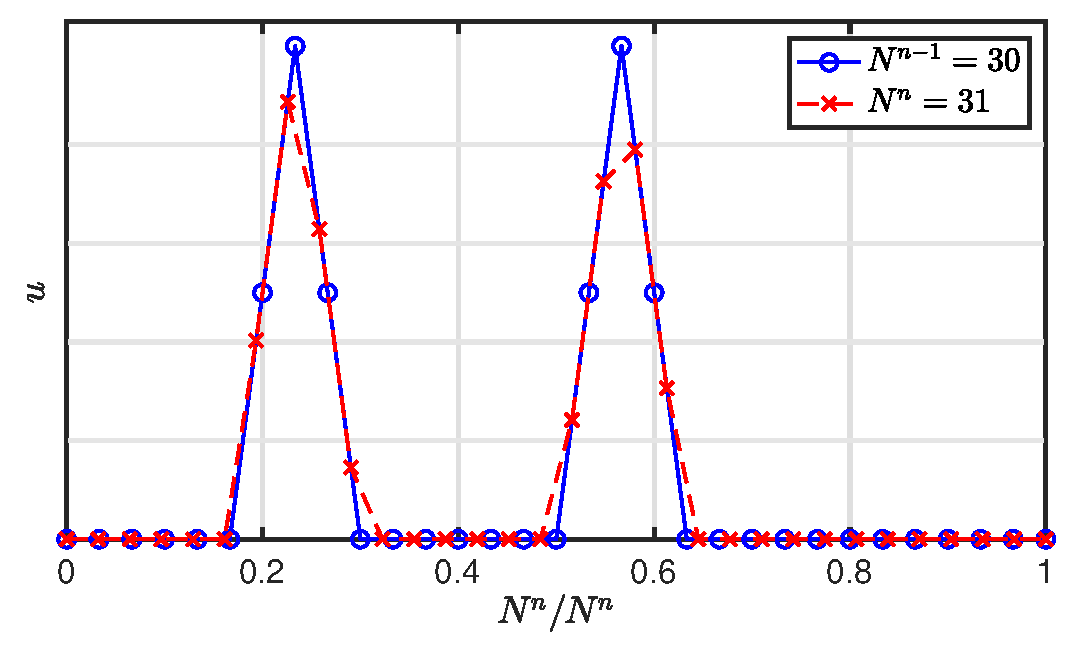
\includegraphics[width=0.5\textwidth]{figures/contributions/dynamicgrid/fullGrid.eps}
\caption{\label{fig:fullGrid}{Upsampling $u$ (with an arbitrary state) using (linear) full-grid interpolation with $N^{n-1} = 30$ and $N^n = 31$. The horizontal axis is normalised with respect to $N^n$.}}
\end{figure} 

An issue that arises using this method is that the Courant number $\lambda$ will slightly deviate from the CFL condition as $c$ changes. Using Eq. \eqref{eq:compactLambda} with $L/ck$ approaching $31$ (from below), the minimum value of $\lambda \approx 30/31 \approx 0.9677$.
%\footnote{Eq. \eqref{eq:orderOfCalcGrid} can be compactly rewritten as $\lambda = \frac{ck}{L}\cdot \text{floor}\left(\frac{L}{ck}\right)$. As $L/ck$ approaches $31$ (from below), $\lambda \approx \frac{30}{31}$.}
This, employing Eq. \eqref{eq:fmax}, has a maximum frequency output of $f_\text{max} \approx 18,475$ Hz. 
%For slightly lower values of $c$, $N = 31$ and $\lambda \approx 1$. 
The Courant number will deviate more for higher values of $c$ and thus lower values for $N$ -- for instance, if $N$ approaches $11$ (from below), $\lambda \approx 10/11 \approx 0.9091$ and $f_\text{max} \approx 16,018$ Hz.

Another problem with full-grid interpolation, is that it has a low-passing effect on the system state, and thus on the output sound. %Figure \ref{fig:fullGrid} shows the biggest changes are in the state are at the locations with the biggest difference between the states of consecutive grid points.
Furthermore, this state-interpolation causes artefacts or `clicks' in the output sound as the method causes sudden variations in the states.  

All the aforementioned issues could be solved by using a (much) higher sample rate and thus more grid points, but this would render this method impossible to work in real time.

\subsection{Adding and removing points at the boundary}\label{sec:addAtBoundary}
To solve the issues exhibited by a full-grid interpolation, points can be added and removed at a single location and leave most points unaffected by the parameter changes. A good candidate for a location to do this is at a fixed (Dirichlet) boundary. The state $u$ at this location is always $0$ so points can be added smoothly. 

As $c$ decreases, $h$ can be calculated according to Eq. \eqref{eq:orderOfCalcGrid} and decreases as well.

This has a physical analogy with tuning a guitar string. Material enters and exits the neck (playable part of the string) at the nut, which in discrete time means grid points appearing and disappearing at one boundary.

To yield smooth changes between grid configurations, an interpolated boundary has been developed, the possibility of which has been briefly mentioned in \cite[p. 145]{theBible}. The Dirichlet condition in Eq. \eqref{eq:contDirichlet} can be extended to be the simply supported boundary condition:
\begin{equation}
    u(x, t) = \frac{\partial^2}{\partial x^2}u(x, t) = 0 \quad \text{where} \quad x = 0, L,
\end{equation}
or, when discretised,
\begin{equation}\label{eq:simplySupportedDiscrete}
    u_l^n = \delta_{xx}u_l^n = 0, \quad \text{where} \quad l = 0, N.
\end{equation}
This means that on top of that the state of the boundary should be $0$, the curvature around it should also be $0$. One can again solve for the virtual grid points at the boundary locations, yielding
\begin{equation}
    u_{-1}^n = -u_1^n \quad \text{and} \quad u_{N+1}^n = -u_{N-1}^n.
\end{equation}
This is visualised in Figure \ref{fig:simplySupportedBound}.

\begin{figure}
    \centering
    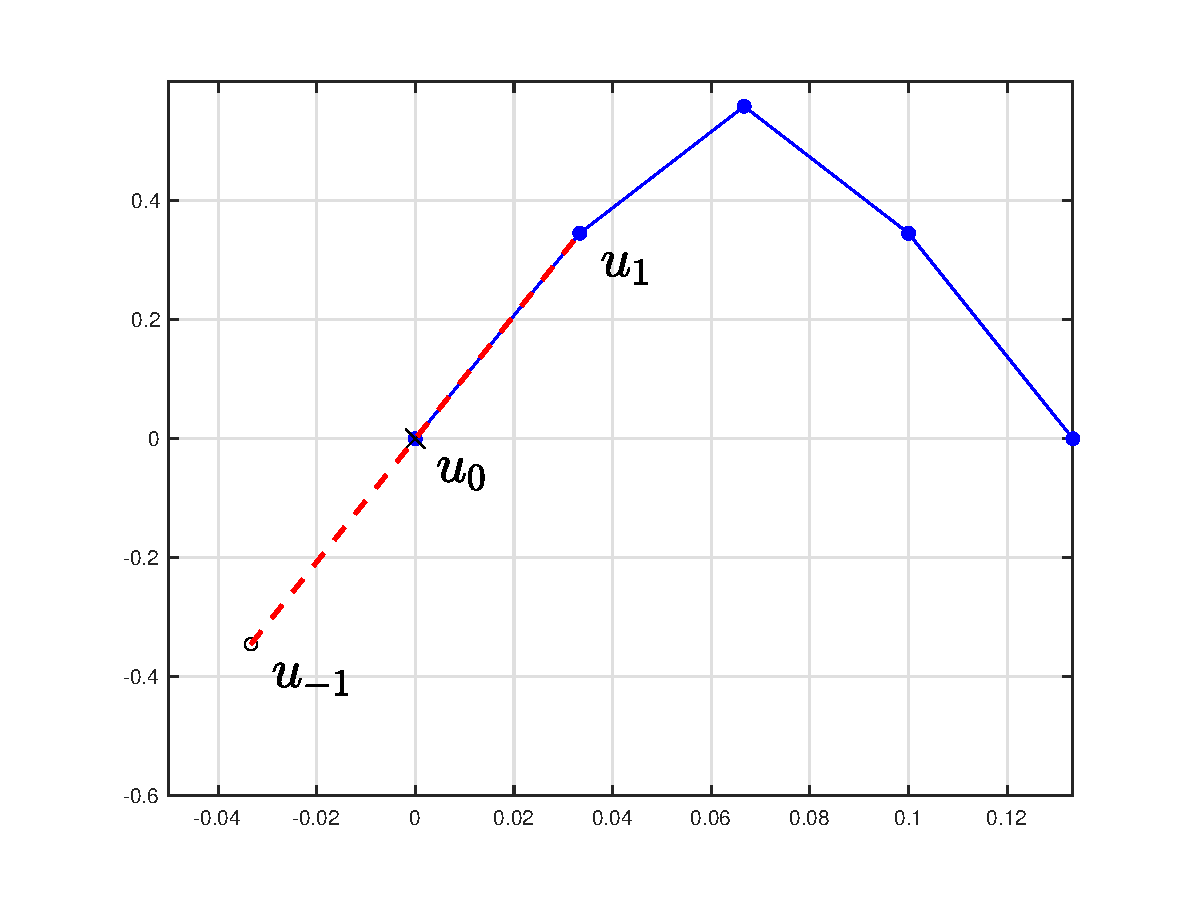
\includegraphics[width=0.7\textwidth]{figures/contributions/dynamicgrid/simplySupportedBoundary.eps}
    \caption{\label{fig:simplySupportedBound}{The simply supported boundary condition: both the state and the curvature at the boundary -- at $l=0$ -- should be $0$.}}
\end{figure} 

If the flooring operation in Eq. \eqref{eq:numberOfIntervals} is removed this introduces a fractional number of grid points.


The by-product of using a fractional $N$ this is that the CFL condition in \eqref{eq:CFL} can now always be satisfied with equality no matter what the wave speed is.

An issue with this method is that removing points is much harder than adding.

their interactions change through a change in the grid spacing and wave speed. This interaction, though, is defined by $\lambda$ which 

\begin{figure}
    \centering
%% \reprintcolumnwidth is the same in preprint and reprint for
%% ease of use for authors:
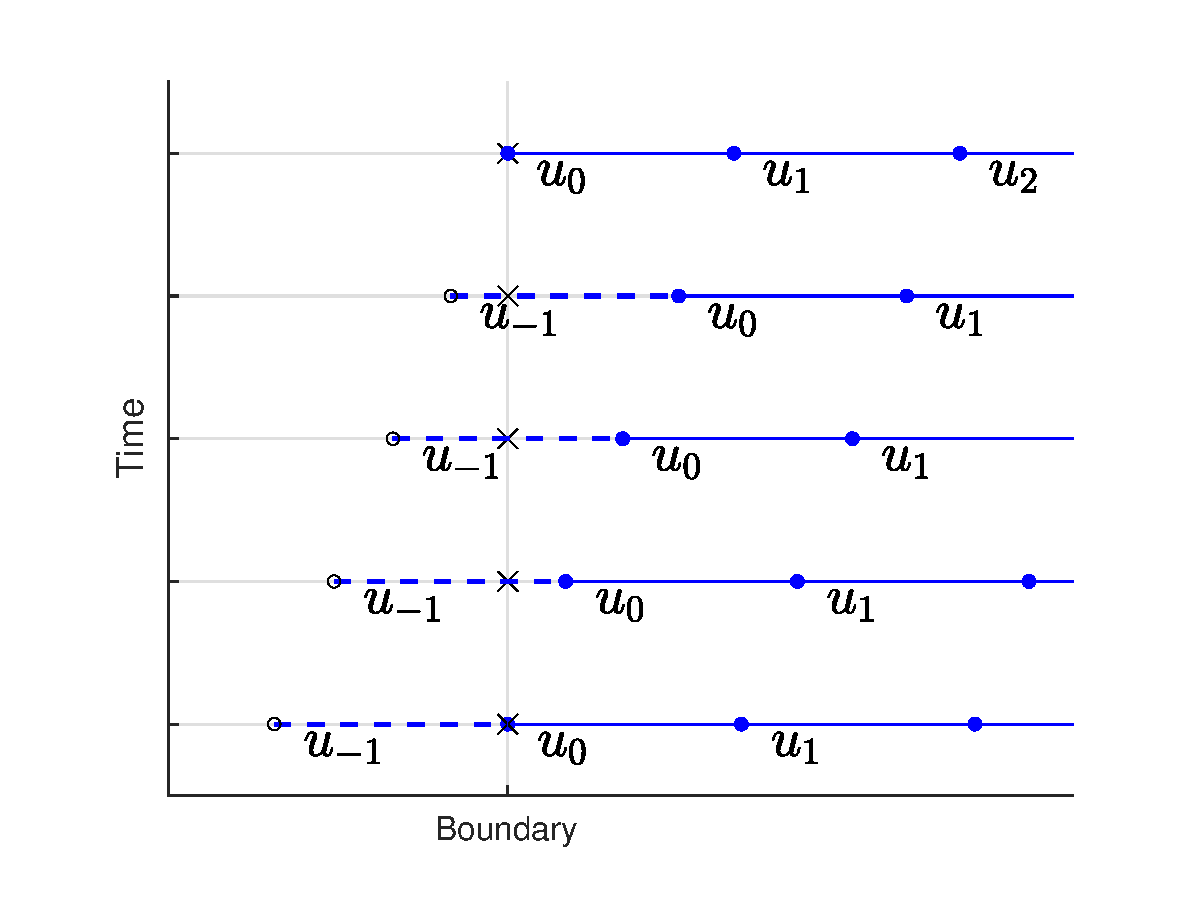
\includegraphics[width=0.7\textwidth]{figures/contributions/dynamicgrid/boundaryGrid.eps}
\caption{\label{fig:changingBoundary}{The grid changing over time}}
\end{figure}

\subsection{Cubic interpolation}

\subsection{Sinc interpolation}


\section{Displacement correction implementation} 
One detail that was not provided in paper \citeP[G], is the impelmentation of the displacement correction.
When the wave speed is increased and points are removed, it is not necessarily true that $u_M = w_0$ at the time of removal and the rigid connection in \eqref{eq:rigid} is violated. On top of the virtual grid point ``generation'' from the interpolation described above, one could add a connection force that is dependent on how close the inner boundaries $u_M$ and $w_0$ are.

Equation \eqref{eq:systemHalfStrings} can be extended to include a spring force between $u_M$ and $w_0$ as
\begin{equation}\label{eq:dispCorrSyst}
    \begin{cases}
        \delta_{tt}u^n &= c^2\delta_{xx}u^n + J(x_{u_M})F\\
        \delta_{tt}w^n &= c^2\delta_{xx}w_0^n - J(x_{w_0})F
    \end{cases}
\end{equation}
with 
\begin{equation}\label{eq:corrForceNoDamp}
    F = \beta \mu_{t\cdot}\eta^n.
\end{equation}
Here,
\begin{equation}\label{eq:etaCorrDef}
    \eta^n \triangleq w_0^n - u_M^n
\end{equation}
is the difference in displacement between the inner boundaries
and $\beta = \beta(\alpha)$ 
acts as a spring coefficient that is a function of the distance between the inner boundaries along the grid, i.e., $\alpha$. Furthermore, the centred temporal averaging operator $\mu_{t\cdot}$ is used in \eqref{eq:corrForceNoDamp} to ensure stability \cite{Bilbao2009Modular}.

We then continue by finding a definition for $\beta$ that is inversely proportional to $\alpha$, i.e., the smaller $\alpha$ is the higher the `correction' effect, ideally approaching an infinite stiffness, or rigid connection, when $\alpha = 0$ and no stiffness when $\alpha \rightarrow 1$. This can be achieved by defining $\beta = \beta(\alpha)$ as
\def\plusEps{+ \epsilon}
% \def\plusEps{};
\def\alfPlusEps{(\alpha \plusEps)}
% \def\alfPlusEps{\alpha}
\begin{equation}\label{eq:betaDef}
    \beta = \frac{1 - \alpha}{\alpha \plusEps},
\end{equation}
with $0<\epsilon \ll 1$ to prevent a division by 0. It will be shown that when calculating the force after expansion, a division by 0 can be prevented and $\epsilon = 0$ will still yield a defined solution. We can observe that when $\alpha = 0$ and the correction effect needs to be at a maximum, $\beta\rightarrow \infty$. When $\alpha \rightarrow 1$, $\beta \rightarrow 0$.

We can also add a damping term to \eqref{eq:corrForceNoDamp} which is also scaled by $\beta$ as
\begin{equation}\label{eq:corrForce}
    F = \beta \left(\mu_{t\cdot}\eta^n +\sigma_0\delta_{t\cdot}\eta^n \right),
\end{equation}
where $\sigma_0$ is the damping coefficient. Then, we can solve for $\eta^{n+1}$ 
\begin{align}
    F &= \beta\left(\frac{1}{2}\left(\eta^{n+1}+\eta^{n-1}\right) + \frac{\sigma_0}{2k}\left(\eta^{n+1}-\eta^{n-1}\right)\right)\nonumber\\
    F&= \left(\frac{\beta (1 + \sigma_0/k)}{2}\right)\eta^{n+1} + \left(\frac{\beta (1 - \sigma_0/k)}{2}\right) \eta^{n-1}\nonumber\\
    \xLeftrightarrow{\mystrut\ \text{Eq. \eqref{eq:betaDef}}\ } \quad \eta^{n+1} &= \left(\frac{2
    \alfPlusEps}{(1+\sigma_0/k)(1-\alpha)}\right)F - \underbrace{\frac{1-\sigma_0/k}{1+\sigma_0/k}}_{r}\eta^{n-1}.\label{eq:etaSolut1}
\end{align}
Using superscript $\text{I}$ to denote an intermediate state describing of $u^{n+1}_M$ and $w^{n+1}_0$ without the connection force (see \eqref{eq:resultOneConnectedPoint}), we also know, through Eq. \eqref{eq:etaCorrDef}, that 

\begin{align}
    \eta^{n+1} &= w_0^\text{I}-\frac{k^2}{h}F-\left(u_M^\text{I}+\frac{k^2}{h}F\right)\nonumber\\
    \eta^{n+1} &= w_0^\text{I} - u_M^\text{I} - \frac{2k^2}{h}F,\label{eq:etaNext}
\end{align}
which can be set equal to \eqref{eq:etaSolut1} and solved for $F$ according to 

\begin{align*}
    \left(\frac{2
    \alfPlusEps}{(1+\sigma_0/k)(1-\alpha)}\right)F - r \eta^{n-1} &= w_0^{I} - u_M^{I}- \frac{2k^2}{h}F\\
    \left(\frac{2h
    \alfPlusEps + 2k^2(1+\sigma_0/k)(1-\alpha)}{h(1+\sigma_0/k)(1-\alpha)}\right)F &= w_0^{I} - u_M^{I}+r\eta^{n-1}\\
    F &= \left(w_0^{I} - u_M^{I}+r\eta^{n-1}\right)\left(\frac{h(1+\sigma_0/k)(1-\alpha)}{2h \alfPlusEps + 2k^2(1+\sigma_0/k)(1-\alpha)}\right).
\end{align*}
It is clear now that no matter the value of $\alpha$, no division by 0 will occur, so $\epsilon = 0$ is still defined. The final equation for $F$ can thus be written as
\begin{equation}\label{eq:finalForce}
    F = \left(w_0^{I} - u_M^{I}+r\eta^{n-1}\right)\underbrace{\left(\frac{h(1+\sigma_0/k)(1-\alpha)}{2h\alpha + 2k^2(1+\sigma_0/k)(1-\alpha)}\right)}_{\Psi}.
\end{equation}
This can then be filled into \eqref{eq:dispCorrSyst} and used to get $u_M^{n+1}$ and $w_0^{n+1}$ respectively. \SWcomment[Using $\alpha = 0$ and $\sigma_0 = 0$ as a test case to see what would happen to the scheme at the inner boundaries when they perfectly overlap (and without damping, just restoring force), we get that $r = 1$ and \eqref{eq:finalForce} becomes
\begin{align*}
    F &= \left(w_0^{I} - u_M^{I}+\eta^{n-1}\right)\left(\frac{h}{2k^2}\right)\\
    \xLeftrightarrow{\mystrut\ \text{Eq. \eqref{eq:etaNext}}\ } \quad F &= \left(\eta^{n+1} + \frac{2k^2}{h}F + \eta^{n-1}\right)\left(\frac{h}{2k^2}\right)\\
    F - F &= \eta^{n+1} + \eta^{n-1}\\
    2\mu_{t\cdot}\eta^n &= 0\\
    \mu_{t\cdot}\eta^n &= 0
\end{align*}
showing that when $\alpha = 0$, the $\eta^n$ should be 0 and thus boils down to a rigid connection.]

\subsubsection{Modal analysis}
Due to the damping that is present in the system, it needs to be written in one-step form. Recalling \eqref{eq:uVecDef} we can write \eqref{eq:dispCorrSyst} in vector-matrix form
\begin{equation}\label{eq:formForOneStep}
    \A \U^{n+1} = \B \U^n + \C\U^{n-1}
\end{equation}
and rewrite to one-step form as \SWcomment[decapitalise u!]
\begin{equation}\label{eq:oneStepFormDynamicGrid}
    \underbrace{\begin{bmatrix}
        \U^{n+1}\\
        \U^n
    \end{bmatrix}}_{\mathbf{W}^{n+1}} = 
    \underbrace{\begin{bmatrix}
        \A^{-1}\B & \A^{-1}\C\\
        \I & \mathbf{0}
    \end{bmatrix}}_{\Q}
    \underbrace{\begin{bmatrix}
        \U^n\\
        \U^{n-1}
    \end{bmatrix}}_{\mathbf{W}^n}
\end{equation}

The most straightforward way to obtain the matrices, is to expand the forces in system \eqref{eq:dispCorrSyst} directly. 
% \begin{equation}
%     \begin{cases}
%         \delta_{tt}u^n &= c^2\delta_{xx}u^n + J(x_{u_M})\frac{\beta}{2}(\eta^{n+1} + \eta^{n-1} + \sigma_0/k (\eta^{n+1} - \eta^{n-1}))\\
%         \delta_{tt}w^n &= c^2\delta_{xx}w_0^n - J(x_{w_0})\frac{\beta}{2}(\eta^{n+1} + \eta^{n-1} + \sigma_0/k (\eta^{n+1} - \eta^{n-1}))
%     \end{cases}
% \end{equation}
% and
Recalling $\U$ from \eqref{eq:uVecDef} (of size $\mathcal{M} = M+M_w$) and including the virtual grid point definitions encapsulated in $\B_2$, we can rewrite the system to
\begin{equation}
    \I\U^{n+1} = \B_2\U^n - \I\U^{n-1} + (\J\boldsymbol{\eta})\frac{\beta k^2}{2}\left((1+\sigma_0/k)\U^{n+1} + (1-\sigma_0/k)\U^{n-1}\right)
\end{equation}
where 
\begin{equation}
    \J = [\mathbf{0}_{M-1}, 1/h, -1/h, \mathbf{0}_{M_w-1}]^T
\end{equation}
where $\mathbf{0}_i$ is a row-vector of zeros with length $i$ and
\begin{equation}
    \boldsymbol{\eta} = [\mathbf{0}_{M-1}, -1, 1, \mathbf{0}_{M_w-1}].
\end{equation}
vectorising the effect of \eqref{eq:etaCorrDef} on $\U$. Note that as $\J$ is a column vector and $\boldsymbol{\eta}$ a row vector, the multiplication of the two yields an $\mathcal{M}\times\mathcal{M}$ matrix.

Then refactoring to the form in \eqref{eq:formForOneStep} and using identity matrix $\I$ with size $\mathcal{M} \times \mathcal{M}$ yields the following matrices
% \begin{equation}
%     \underbrace{\left(\I - \frac{\beta k^2 (1+\sigma_0/k)}{2}\J\boldsymbol{\eta}\right)}_{\A}\U^{n+1} = \underbrace{\mathbf{B}_2}_{\B}\U^n +\underbrace{\left(- \I - \frac{\beta k^2 (1-\sigma_0/k)}{2}\J\boldsymbol{\eta}\right)}_{\C} \U^{n-1}
% \end{equation}

\begin{equation}
    \A = \I - \frac{\beta k^2 (1+\sigma_0/k)}{2}\J\boldsymbol{\eta}, \qquad \B = \mathbf{B}_2, \qquad \text{and} \qquad \C = -\left(\I - \frac{\beta k^2 (1-\sigma_0/k)}{2}\J\boldsymbol{\eta}\right)
\end{equation}
Although substituting these definitions into \eqref{eq:oneStepFormDynamicGrid} gives an identical result to the matrix definitions above (comparisons show a difference between the $\Q$ matrices around machine precision), $\beta$ can still go to infinity. In this case, $\epsilon \neq 0$ in \eqref{eq:betaDef}. 

\section{%Modal 
Analysis and experiments}
\subsection{Interpolation technique}
\subsection{Interpolation range}
\subsection{Location}
... where to add and remove points

Using the whole range, we can still add/remove points at the sides. 

\section{Discussion and conclusion}\label{sec:conclusion}

\pagebreak
{\small\bibliographystyle{IEEEtranS}\bibliography{bib/mybib}}

%backmatter
% \appendix
% \part{Papers}
% \chapter*{Paper Errata}
Here, some errors in the published papers will be listed:
\\
\textbf{Real-Time Tromba \citeP[D]}: 
\begin{itemize}
    \item The minus sign in Eq. (28) (and thus Eqs. (31) and (35)) should be a plus sign.
    \item $\sigma_{1,\text{s}}$ in Eq. (21) should obviously be $\sigma_{1,\text{p}}$
    \item the unit of the spatial Dirac delta function $\delta$ should be m$^{-1}$
\end{itemize}
%
\textbf{DigiDrum \citeP[F]}: 
\begin{itemize}
    \item $\sigma_0$ and $\sigma_1$ should be multiplied by $\rho H$ in order for the stability condition to hold.
    \item stability condition is wrong. Should be: 
    \begin{equation}
        h \geq \sqrt{c^2k^2 + 4\sigma_1k + \sqrt{(c^2k^2+4\sigma_1k)^2 + 16\kappa^2k^2}}
    \end{equation}
    \item Unit for membrane tension is N/m.
\end{itemize}
%
\textbf{Dynamic grids \citeP[G]}
\begin{itemize}
    \item Reference in intro for `recently gained popularity' should go to \cite{Bilbao2019CMJa} \\
    \textit{Note: not really an error, but should be changed before resubmission}
\end{itemize}

\titleformat{%command
  \chapter
}[%shape
display%
]{%format
  \normalfont\huge 
}{%label
  \begin{center}\color{aaublue}\chaptertitlename\ \thechapter\end{center}
}{%style
  1cm
}{%code before title
  \thispagestyle{empty}\begin{center}\Large
[%code after title
]
  \end{center}}

% \includepaper{papers/paperA/paperA}
% \includepaper{papers/paperB/paperB}
\end{document}
